% small.tex

\documentclass{beamer}
\usepackage{graphicx}
\usepackage{multirow}
\usepackage{tabularx}  
\usepackage{lingmacros}

\renewcommand{\vec}[1]{\mathbf{#1}}
\graphicspath{./images/}
\usetheme{Copenhagen}

\newcommand{\sentenceexample}[1]{{\small\enumsentence{#1}}}

\title{Shallow-transfer rule-based machine translation for the Western group of South Slavic languages}
\author{
	Hrvoje Peradin, Filip Petkovski and Francis Tyers
}

\date{May 27, 2014}
\begin{document}
% --------------------------- Title Page --------$------------------ %
\begin{frame}
  \titlepage
\end{frame}

% --------------------------- Europe -------------------------- %
\begin{frame}{The Balkan peninsula}
\begin{center}
	\begin{figure}
	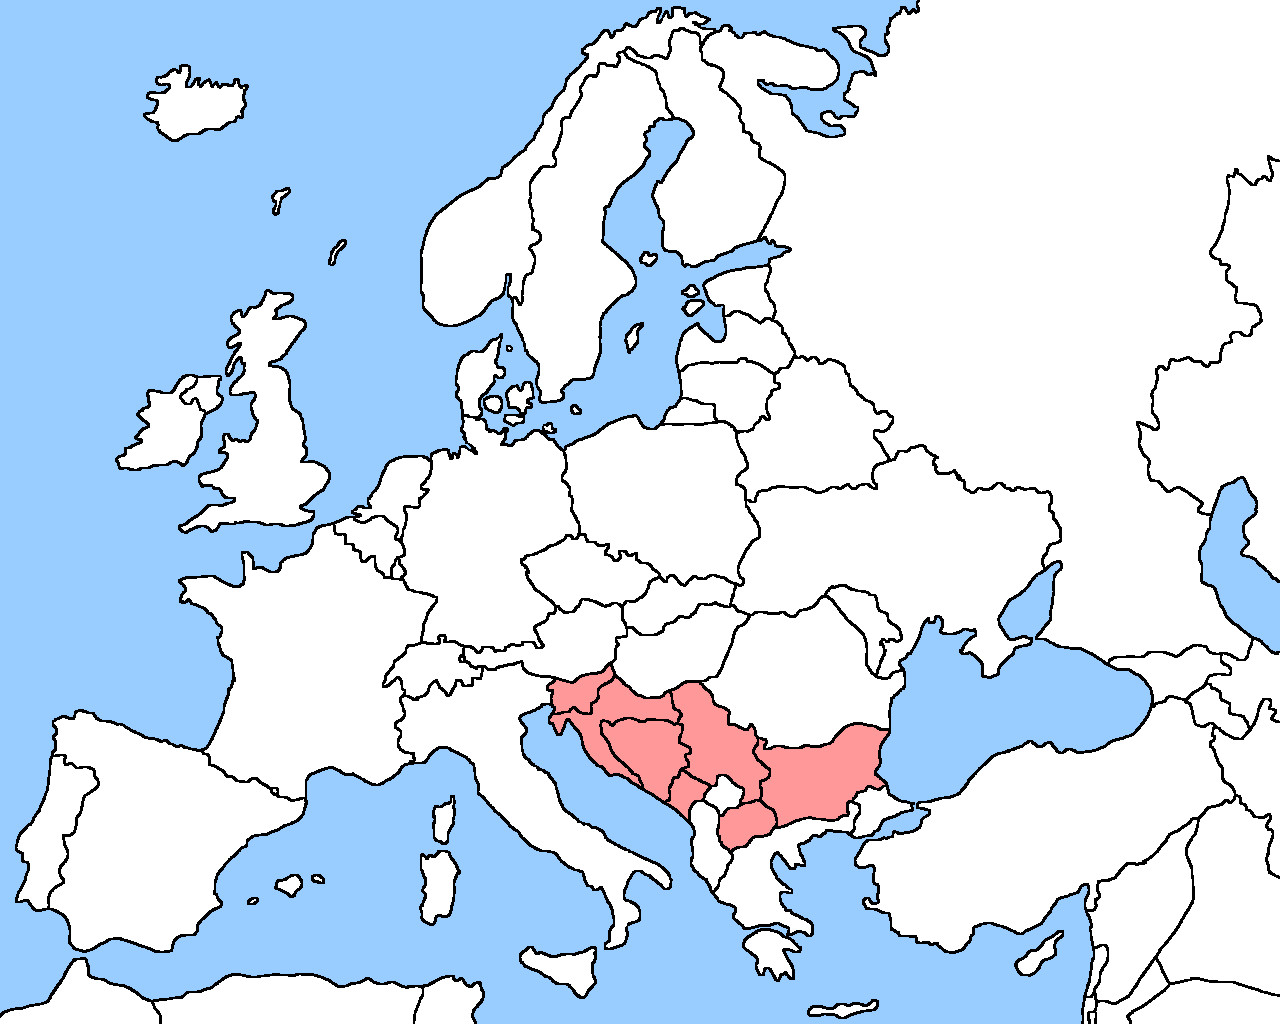
\includegraphics[width=0.7\textwidth]{images/europe.jpg}
	\label{fig:1}
	\caption{The Balkan peninsula}
	\end{figure}
\end{center}
\end{frame}

% --------------------------- Balkans -------------------------- %
\begin{frame}{The Balkan peninsula}
\begin{center}
	\begin{figure}
	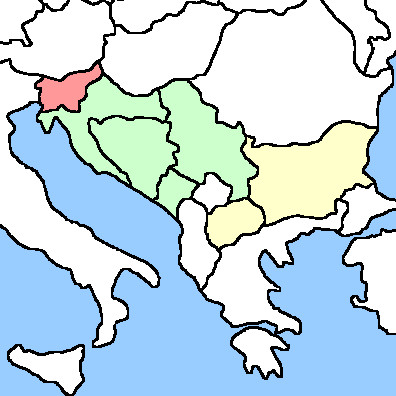
\includegraphics[width=0.6\textwidth]{images/balkans.jpg}
	\label{fig:1}
	\caption{The Balkan peninsula}
	\end{figure}
\end{center}
\end{frame}


% --------------------------- Slide 4 -------------------------- %
\begin{frame}{Introduction}

\begin{center}
	\begin{figure}
	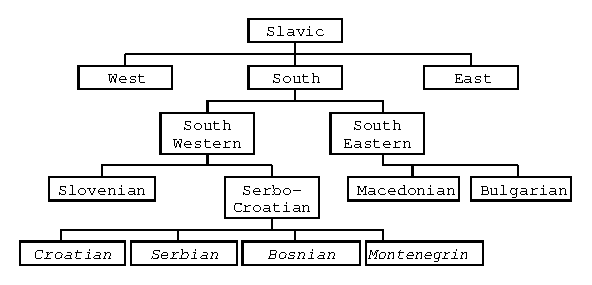
\includegraphics[width=0.8\textwidth]{images/chart.eps}
	\label{fig:1}
	\caption{A traditional division of the South-Slavic languages. All four standard varieties of Serbo-Croatian (Bosnian, Croatian,
Montenegrin, and Serbian) are based on the shtokavian dialect.}
	\end{figure}
\end{center}
\end{frame}

% --------------------------- Slide 5 -------------------------- %
\begin{frame}{The Apertium platform}
\begin{figure}
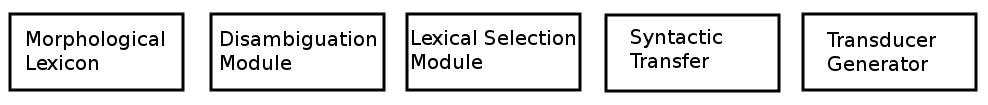
\includegraphics[width=\textwidth]{images/apertium.png}
\caption {Basic Apertium setting}
\end{figure}
The Apertium platform is a modular machine translation system.
The core setup consists of:
\begin{itemize}
\item A letter transducer morphological lexicon
\item Morphological disambiguation module
\item Lexical selection module
\item Syntactic transfer module
\item A letter transducer generator
\end{itemize}
\end{frame}

% --------------------------- Slide 6 -------------------------- %
\begin{frame}{Resources}
Several resources were used extensively throughout the development process:
\begin{itemize}
\item On the Serbo-Croatian side we used the Croatian Language Portal (Hrvatski jezi\v{c}ni portal)
\item The Amebis Besana flective lexicon and other resources were used for the Slovenian side
\item EUDict was used as the main resource for the bilingual dictionary

\end{itemize}
\end{frame}


% --------------------------- Slide 7 -------------------------- %
\begin{frame}{Morphological analysis and generation}
\begin{itemize}

\item The basis for this language pair are the morphological lexicons for Serbo-Croatian and Slovenian developed during Google Summer of Code 2011
\item The Serbo-Croatian dictionary was developed as part of a Serbo-Croatian--Macedonian pair
\item The Slovenian dictionary was developed within a Slovenian--Spanish project
\item Both lexicons had to be synchronized and trimmed down since they were developed with different tagsets and frequency lists 

\end{itemize}
\end{frame}

% --------------------------- Slide 8 -------------------------- %
\begin{frame}{Disambiguation}
\begin{itemize}

\item Satisfactory results were not obtained with the cannonical statistical tagger used in Apertium language pairs
\item Constraint Grammar rules developed for the Serbo-Croatian -- Macedonian project were reused on the Serbo-Croatian side 
\item We relied solely on Constraint Grammar, which chooses the first output analysis in the case of remaining ambiguity
\item Many of the rules developed for Serbo--Croatian were reused for Slovenian

\end{itemize}
\end{frame}

% --------------------------- Slide 9 -------------------------- %
\begin{frame}{Lexical transfer}
\begin{itemize}

\item Lexical transfer was done using an \emph{lttoolbox} letter transducer and a bilingual dictionary.
\item Additional paradigms were added for simple tagset mismatches which could be easily resolved in this stage
\begin{itemize}
	\item One example are cases when the adjective on one side is synthetic, and on the other analytic (\emph{zdravije} vs \emph{bolj zdravo})
\end{itemize}
\end{itemize}
\end{frame}

% --------------------------- Slide 10 -------------------------- %
\begin{frame}{Lexical selection}
\begin{itemize}
\item Due to a lack of a parallel corpus, Lexical selection was done based on hand-written rules
\item For cases not covered by our hand-written rules, the default translation from the bilingual dictionary was chosen
\item The lexical selection module was used mainly for:
\begin{itemize}
	\item Phonetics-based lexical selection: words that differ in a single phoneme, like \emph{to\v{c}no} and \emph{ta\v{c}no} (accurate)
	\item Croatian months have Slavic-derived names and differ from the original Latin names (\emph{sije\v{c}anj} -- January)
\end{itemize}
\end{itemize}
\end{frame}


% --------------------------- Slide 11 -------------------------- %
\begin{frame}{Syntactic transfer}
\begin{itemize}
\item Most transfer rules were written to:
\begin{itemize}
\item Bridge tagset differences
\begin{itemize}
	\item 
  \sentenceexample{
Gledal bom
$\leftrightarrow$ 
Gledat \'{c}u
[watch{\sc.lp.m.sg}][be{\sc.clt.p1.sg}] 
$\leftrightarrow$ 
[watch{\sc.inf}][will{\sc.clt.p1.sg}]
(I will watch.)
}

\end{itemize}
\item Cover different word orders
\end{itemize}
\end{itemize}
\end{frame}

% --------------------------- Slide 12 -------------------------- %

\begin{frame}{Evaluation}
\begin{itemize}
\item Lexical coverage, qualitative and quantitative analysis was performed
\item Lexical coverage tested using existing free corpora
\begin{itemize}
\item SETimes
\item EuroParl
\end{itemize}
\item Quantitative evaluation performed on 100 postedited sentences from the Slovenian news portal Delo
\end{itemize}
\end{frame}

% --------------------------- Slide 13 -------------------------- %

\begin{frame}{Evaluation | Lexical Coverage}
\begin{itemize}
\item Lexical coverage was measured using SETimes and Europarl
\end{itemize}
% Hrvatski -> Slovenski
\begin{table}
\begin{tabular}{lrr}

\textbf{Language} & \textbf{SETimes} & \textbf{Europarl}\\
\hline
Serbo-Croatian & 85.41\% & -- \\
Slovenian &  -- & 95.50\%\\
\hline
\end{tabular}
\caption{ Statistics on number of lexicon entries for each of the
dictionaries in the system }
\label{table:coverage}
\end{table}


\begin{table}
\begin{center}
\begin{tabular}{|l|rrr|}
\hline
\textbf{Dictionary} & \textbf{Paradigms} & \textbf{Entries} & \textbf{Forms} \\
\hline
Serbo-Croatian &  1,033 & 13,206 & 233,878 \\
Slovenian &  1,909 & 13,383 & 147,580 \\
\hline
Bilingual &  69 &  16,434 & -- \\
\hline
\end{tabular}
\caption{Statistics on number of lexicon entries for each of the dictionaries in the 
   system.}
\label{table:lexicons}
\end{center}
\end{table}



\end{frame}

% --------------------------- Slide 14 -------------------------- %

\begin{frame}{Evaluation | Quantitative }
\begin{itemize}
\item Performed on 5 news articles from Delo
\item WER calculated on post edited translations
\item Apertium's results were compared to Google Translate's ones
\end{itemize}

% cp /path/to//apertium//trunk/apertium-eval-translator/WER.pl /path/to/bin
% perl apertium//trunk/apertium-eval-translator/bootstrap_resampling.pl -n 1000 -e /path/to//apertium//trunk/apertium-eval-translator/wer.sh -s SOURCE_FILE -t TEST_FILE -r REF_FILE

\begin{table*}
\begin{center}
\begin{tabular}{|l|r|rr||rr|}
   \hline
  \multirow{2}{*}{\textbf{Article}}  & \multirow{2}{*}{\textbf{Words}} & \multicolumn{2}{|c||}{\textbf{\%~OOV}} & \multicolumn{2}{c|}{\textbf{WER}}\\\cline{3-6}
                    &                & Apertium & Google &  Apertium & Google \\
   \hline
   \hline
  \texttt{maraton}  & 243            & 16.8     & --     & \textbf{[42.85, 47.92]} & [64.39, 74.56] \\
  \texttt{sonce}    & 169            & 17.7     & --     & \textbf{[32.65, 45.33]}    & [47.27, 58.62] \\
  \texttt{merkator} & 414            & 16.9     & --     & \textbf{[38.78, 48.14]}     & [56.13, 70.30] \\
  \texttt{volitve}  & 229            & 13.9     & --     & [37.81, 53.36]      & [46.66, 62.67] \\
%  \texttt{jame}     & 994            & 14.9     & --     & ??      & [57.28, 67.65] \\
                                                           % 49.57	
  \hline
  \hline
  \texttt{maraton}  & 245            & 37.7     & --     & [52.78, 56.25]           & [45.58, 63.87]\\
  \texttt{sonce}    & 171            & 17.5     & --     & [47.50, 62.79]    & [32.10, 58.49] \\
  \texttt{merkator} & 424            & 12.9     & --     & [45.78, 56.56]    & [48.46, 64.15] \\
  \texttt{volitve}  & 226            & 16.8     & --     & [47.00, 58.44]    & [38.09, 58.10]\\
%  \texttt{jame}     & 1,005          & 15.9     & --     & [??, ??]              & [??,??]\\

  \hline
\end{tabular}
 \caption{Results for Word Error Rate (WER) in the Slovenian$\rightarrow$Serbo-Croatian direction (top) and Serbo-Croatian$\rightarrow$Slovenian (bottom). Scores in bold show a statistically significant improvement over the other system according to bootstrap resampling at $p = 0.95$.}
\label{table:quantitative1}
\end{center}
\end{table*}



\end{frame}

% --------------------------- Slide 15 -------------------------- %

\begin{frame}{Evaluation | Qualitative }
\begin{itemize}
\item Big problems caused by incompleteness of dictionaries
\item OOV words cause problems with disambiguation and transfer, breaking context
\item Low number of disambiguation rules for Slovenian since it was based on the Serbo-Croatian instance
\item Loose grammar on both sides causes difficulties writing transfer rules
\item The lexical selection module is the least developed one
\end{itemize}
\end{frame}


\begin{frame}{Evaluation | Future Work }
\begin{itemize}
\item Improve coverage of dictionaries
\item Develop the Slovenian constraint grammar
\item Work on other Slavic language pairs (Serbo-Croatian -- Russian) and improve existing ones (Serbo-Croatian -- Macedonian)
\item Add Montenegrin language to the \emph{hbs} group once the standard is agreed on

\end{itemize}
\end{frame}

\begin{frame}{ The end }
\begin{center}
\Large{
Thank you for your attention! \\
Tack för uppmärksamheten! \\
Hvala na pozornosti! \\
!`Gracias por su atenci\'{o}n! 
}
\end{center}

\end{frame}


\end{document}
